\section{Implementacja}
Używana przez nas biblioteka \textit{MultiAgent-Gym} domyślnie dostarcza przykładowe
środowiska, które reprezentują różnego rodzaju problemy (w tym przypadku są to różnego
rodzaju gry, w których agenci konkurują ze sobą).

Do naszych celów konieczne było utworzenie nowego środowiska, korzystając z bazowych elementów biblioteki.
Najistotniejszą zmianą jest sposób uczenia poszczególnych agentów. W przypadku domyślnego
przykładu gry \textit{Predator and Prey} agentami są jedynie łowcy, podczas gdy ofiary poruszają
się losowo. Chcieliśmy jednak zamodelować sytuację dwóch konkurujących zespołów, zatem wprowadziliśmy
następujące modyfikacje:
\begin{itemize}
    \item Każdy aktor jest oddzielnym agentem, z własnym zestawem parametrów
    \item Każdy agent otrzymuje indywidualnie obliczaną nagrodę na podstawie określonych kryteriów
    \item Każdy agent komunikuje się z innymi, przekazując informacje o aktualnie obserwowanym otoczeniu,
          co pozwala całej grupie na podejmowanie decyzji w oparciu o wspólną wiedzę (Rys. \ref{fig:agent_view}).
\end{itemize}
\begin{figure}[H]
  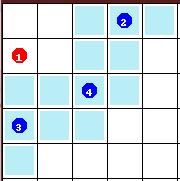
\includegraphics[width=\linewidth]{images/agent_view.png}
  \caption{Obszar widziany przez agenta nr 4.}
  \label{fig:agent_view}
\end{figure}


Niezależnie od siebie agenci podejmują następujące decyzje:
\begin{itemize}
    \item Wykonują optymalny ruch na podstawie obserwacji
    \item Uczą się na podstawie każdej podjętej akcji, obserwacji konsekwencji swoich działań 
          przed i po wykonaniu ruchu oraz otrzymanej nagrodzie
\end{itemize}



